\subsubsection{Implémentation et comparaison des stratégies de balayage}

\subparagraph{(a) Choix de la distribution jointe $Q_Y$}
Nous définissons une distribution jointe sur deux variables 
$Y_1, Y_2 \in \{1, 2, 3, 4\}$ par la matrice $Q_Y \in \mathbb{R}^{4 \times 4}$ suivante :
\begin{equation}
    [Q_Y]_{i,j} = \frac{i+j}{80}, \quad \forall i,j \in \{1, \dots, 4\}
\end{equation}
Cette distribution respecte la condition de positivité ($Q_Y > 0$), 
ce qui garantit que la chaîne de Markov est \textbf{irréductible} et \textbf{apériodique}. 
Ces deux conditions assurent, selon la théorie du point 1, que l'algorithme de Gibbs convergera 
vers l'unique distribution stationnaire $Q_Y$.

\subparagraph{(b) Réalisation par balayage aléatoire (Algorithme 1)}
Nous avons généré une chaîne de $50\,000$ itérations en choisissant à chaque étape 
l'indice de la variable à mettre à jour uniformément dans $\{1, 2\}$. Les tirages selon les 
lois conditionnelles $P(Y_1 \mid Y_2)$ et $P(Y_2 \mid Y_1)$ ont été effectués via la méthode 
de la transformée inverse. La Figure \ref{fig:gibbs_comp} montre que les fréquences empiriques 
épousent parfaitement les valeurs théoriques de $Q_Y$.

\subparagraph{(c) Balayage systématique et conclusion}
L'expérience a été répétée en utilisant un balayage systématique 
(mise à jour de $Y_1$ puis de $Y_2$ à chaque itération). Les résultats obtenus 
sont statistiquement identiques à ceux du balayage aléatoire. 

\begin{figure}[ht]
    \centering
    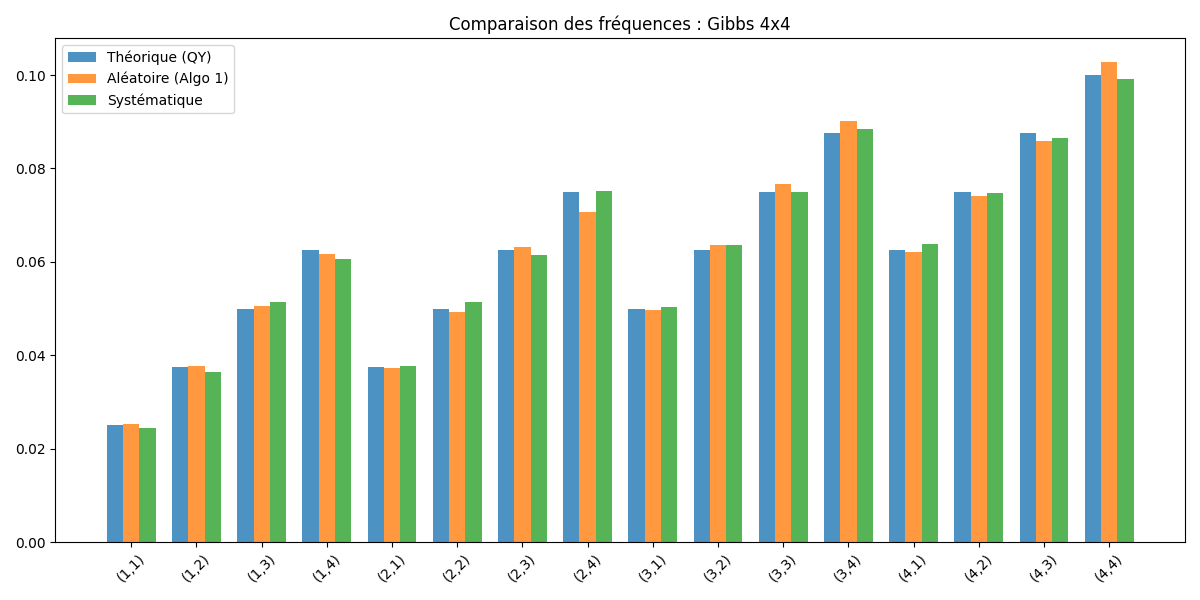
\includegraphics[width=0.9\textwidth]{./images/comparaison_gibbs.png}
    \caption{Comparaison des fréquences d'états pour les deux stratégies de balayage de Gibbs par rapport à la distribution cible.}
    \label{fig:gibbs_comp}
\end{figure}

En conclusion, les deux methodes de balayage (aléatoire et systématique) 
conduisent à des résultats similaires en termes de convergence vers la distribution cible $Q_Y$.